\documentclass[conference]{IEEEtran}
\IEEEoverridecommandlockouts
% The preceding line is only needed to identify funding in the first footnote. If that is unneeded, please comment it out.
\usepackage{cite}
\usepackage{amsmath,amssymb,amsfonts}
\usepackage{algorithmic}
\usepackage{graphicx}
\usepackage{textcomp}
\usepackage{xcolor}
\def\BibTeX{{\rm B\kern-.05em{\sc i\kern-.025em b}\kern-.08em
    T\kern-.1667em\lower.7ex\hbox{E}\kern-.125emX}}
    
\begin{document}

\title{Satellite Constellation Simulation Research\\
\footnotesize \textsuperscript{*}}

\author{\IEEEauthorblockN{Timothy Holden}
\IEEEauthorblockA{\textit{Department of Electrical and Computer Engineering} \\
\textit{University of Colorado Colorado Springs}\\
Colorado Springs, USA \\
tholden@uccs.edu}}

\maketitle

\begin{abstract}
Selecting the appropriate orbit for a satellite communications system is vital to ensure optimal utilization of the intended service. The trade-offs specific to orbital selection have a significant impacts on the systems cost and performance throughout the entire life cycle of the system. In this article I propose the geosynchronous orbital selection for a mm-wave high-throughput system in support of DOD Intelligence, Surveillance, and Reconnaissance missions sets.\\
\end{abstract}

\begin{IEEEkeywords}
Geosynchronous, apogee, perigee, semi-major axis, eccentricity, inclination, periapsis, node, mm-wave, prograde
\end{IEEEkeywords}

\section{Introduction}
A geosynchronous orbit is a high Earth orbit that allows satellites to match Earth's rotation. Located at 22,236 miles (35,786 kilometers) above Earth's equator, this position is ideal for monitoring weather, communications and surveillance. The International Telecommunication Union (ITU) assigns slots for geosynchronous orbit and settles disputes between countries about slots. For disposal, it is considered good practice to move satellites at or near end-of-life into a "graveyard" orbit above geosynchronous orbit before they run out of fuel so to open the slot for follow-on systems \cite{b1}. A geosynchronous orbit (GEO) is a prograde, low \textbf{inclination} orbit about Earth having a period of 23 hours 56 minutes 4 seconds \cite{b2}. Geosynchronous orbits (GEO) are circular orbits around the Earth having a period of 24 hours. A geosynchronous orbit with an inclination of zero degrees is called a geostationary orbit. A spacecraft in a geostationary orbit appears to hang motionless above one position on the Earth's equator. For this reason, they are ideal for some types of communication and meteorological satellites. A spacecraft in an inclined geosynchronous orbit will appear to follow a regular figure-8 pattern in the sky once every orbit. To attain geosynchronous orbit, a spacecraft is first launched into an elliptical orbit called a geosynchronous transfer orbit (GTO). The orbit is then circularized by firing the spacecraft's engine at apogee \cite{b3}.

\section{Orbital Elements}
To mathematically describe an orbit there are six (6) quantities which must be calculated. The quantities are called orbital elements, also known as Keplerian elements named after Johannes Kepler (1571-1630). These six elements are the semi-major axis, eccentricity, inclination, argument of periapsis, time of periapsis passage, and celestial longitude of ascending node. The semi-major axis is one-half of the longest line through the center of an ellipse which represents a satellites mean distance from the body it is orbiting. Eccentricity is the quantitative measure describing the deviation of an orbital curve from circularity. Inclination is a measure of angular distance of an orbital plane from the Earth's equator. The argument of periapsis represents the angular distance of the periapsis (shortest distance between satellite and Earth) from the ascending node. The time of periapsis passage is the time in which a satellite moves through its point of periapsis. The celestial longitude is analogous to longitude on Earth, measured in degrees, counterclockwise from zero with zero longitude being in the direction of the vernal equinox.

\section{Advantages of GEO}
Due to the height of satellites in geosynchronous earth orbit a significant geographical area can be covered by a single satellite. More specifically, only three satellites are required to provide coverage for the entire earth with the exception of the north and south polar regions. Satellites in GEO remain in a fixed position enabling 24/7 access from ground stations eliminating the need for inter-satellite handovers. Lastly, satellites in geosynchronous earth orbit eliminate the need to compensate for doppler shifts due to satellite being stationary relative to the earth \cite{b4}. 

\section{Disadvantages of GEO}
Due to the height of satellites relative to ground stations, there is considerable latency of approximately 240 milliseconds (round-trip) due to the radial distance of the satellite from earth ground stations. Therefore, despite the increased coverage with less satellites, these satellites are not ideal for time-critical operations such as real-time voice, image, and video communication systems. Furthermore, the increased distance also results in the need of more complex and costly electronics such as low-noise amplifiers and signal processing equipment on the payload as well as the ground stations. Lastly, due to the fixed position of satellites in geosynchronous earth orbit and the curvature of the earth, communications of $\pm$ 70 degrees latitude is not possible \cite{b4}. 

\section{Associated Costs}
According to an article written by Dr. Thomas Withington titled "Space on Budget" the cost could be up to \$30,000 per kilogram (2.2 pounds) to launch a satellite into GEO or GSO. A reasonable expectation with respect to the weight of the payload would be consistent with the Advanced Extremely High Frequency (AEHF) and/or Wideband Global SATCOM (WGS) payloads which is approximately 6,000 kilograms \cite{b6} \cite{b7}. At this weight the cost to launch one of these satellites into orbit would be approximately \$180 million. Furthermore, the cost of each satellite for advanced systems, such as the high-throughput mm-wave satellite proposed, would be somewhere between the cost of a WGS system (approx. \$300 million)\cite{b6} and an AEHF system (approx. \$580 million)\cite{b7} which would be approximately \$440 million per satellite. In addition to the logistics of building and launching the satellite, the cost to operate and sustain the satellite in orbit would be approximately \$1,000,000 per year, as well as the cost of bandwidth which begins at approximately \$1,500 per MHz. However, given the lack of congestion at W-band (75GHz-110GHz) frequencies, the proposed system would be less than auctioned prices for bandwidths at the congested UHF (300MHz-3GHz), SHF (3GHz-30GHz), and EHF (30GHz-300GHz) frequency ranges.  

\section{Atmospheric Windows}
Selecting an operating range is a combination of balancing cost and performance with available bandwidths specific to the systems capabilities. Below 30 MHz, the ionosphere, at altitudes from around 100 to 500 km, absorbs and reflects signals. The following is a description of frequency bands:
\begin{figure}[h]
\centerline{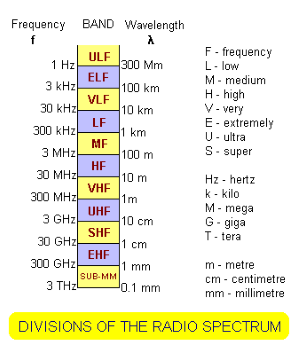
\includegraphics{divisions_of_radio_spectrum300.png}}
\caption{Division of Radio Spectrum}
\label{fig:1}
\end{figure}
\\Above 30 GHz, the lower atmosphere or troposphere, below 10 km, absorbs radio signals due to oxygen and water vapor. Even between 20 and 30 GHz, there are some absorption bands that must be avoided. However, there exists an atmospheric window in the W-band (75GHz-110GHz). The majority of contemporary satellite communication systems today utilize the UHF, SHF and the lower-end of the EHF spectrums. However, with lower frequencies such as UHF comes congestion limiting available bandwidth which inherently limits available throughput.\\
Higher frequencies enable greater bandwidth which translates to increased throughput. For example, the entire bandwidth of the UHF spectrum is 2.7GHz, the SHF spectrum has 27GHz, and the EHF spectrum has 270GHz. As you can see, the available bandwidth increases by a factor of 10 which each band. Therefore, the increase in bandwidth enables additional data to be modulated onto the carrier wave for transmission. The proposed system would utilize the atmospheric window at 100GHz on the uplink and 94GHz on the downlink. The W-band frequency range has great appeal due to the lack of congestion, open atmospheric window, and extremely high throughput possible. The following is a depiction of the atmospheric window with a vertical line at 94GHz which would be used on the downlink:
\begin{figure}[h]
\centerline{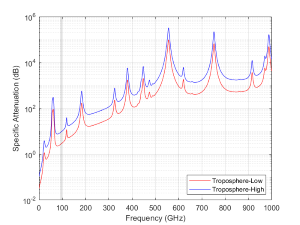
\includegraphics{copyMATLAB300x225.png}}
\caption{Atmospheric Window at 94GHz}
\label{fig:2}
\end{figure}

\section{Simulation}
MATLAB was the software tool used to display the constellation in geosynchronous earth orbit. The orbital elements used in the simulation are the two-line element (TLE) files for the Advanced Extremely High Frequency (AEHF) constellation from the Space-Track.org website. The following is a snapshot of the constellation created using the AEHF orbital elements with the satellite footprints displayed circling the earth perpendicular to the line-of-sight of the satellites relative to the ground station created at the UCCS campus latitude and longitude coordinates acquired through Google Maps:
\begin{figure}[h]
\centerline{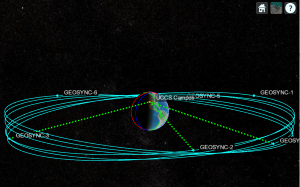
\includegraphics{constellation1copy.png}}
\caption{Geosynchronous Earth Orbit Simulation Snapshot}
\label{fig:3}
\end{figure}
\\\\\\\\The following is an aerial view of the constellation in the simulation displaying both the position of the individual orbital elements in geosynchronous earth orbit as well as the beam footprints:
\begin{figure}[h]
\centerline{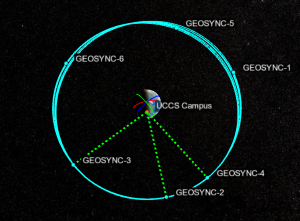
\includegraphics{constellation2copy.png}}
\caption{Geosynchronous Earth Orbit Simulation Aerial View}
\label{fig:4}
\end{figure}

\section{Conclusions}
When compared to other orbits the geosynchronous earth orbit has the advantage of maintaining continuous coverage and providing multi-point simultaneous service over a large geographical area. The low earth orbit has negligible latency but requires significantly more satellites to adequately cover a small region with continuous service. LEO is an optimal solution for time-critical applications such as real-time image and video processing and streaming. The medium earth orbit has significantly less latency than GEO but still requires handoffs and compensation for doppler shift but has significantly better geographical coverage than LEO satellites. The MEO constellation is an optimal solution for services that require low-latency but not real-time image and video processing over a relatively large coverage area and the complexities introduced by handoffs and compensation for doppler shift in the onboard digital signal processing payload do not outweigh the benefits of placing the satellite in GEO despite the increased latency. Another constellation typically used for coverage in the polar regions is the Highly Elliptical Orbit (HEO) which is typically only used for this purpose and only provides service over a small duration of its orbital period. The following are examples of the LEO constellation using Starlink TLE files and the MEO constellation using currently operational GPS TLE files also acquired from the Space-Track.org website:
\begin{figure}[h]
\centerline{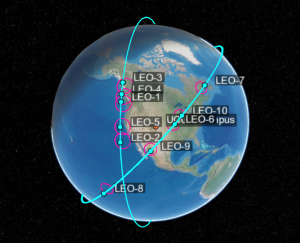
\includegraphics{constellation3copy.png}}
\caption{Example of Low Earth Orbit}
\label{fig:5}
\end{figure}
\begin{figure}[h]
\centerline{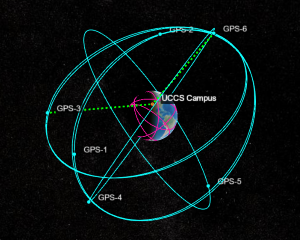
\includegraphics{constellation4copy.png}}
\caption{Example of Medium Earth Orbit}
\label{fig:6}
\end{figure}
\\\\In conclusion, the orbital selection specific to a satellite constellation is a balance of cost and performance. Each constellation has its advantages and disadvantages, but due to the complexities introduced as a result of mm-wave W-band communications, satellites in relatively fixed positions are ideal. Furthermore, the additional coverage provided by significantly fewer satellites by which to provide high throughput communications is also ideal. 

\begin{thebibliography}{00}
\bibitem{b1} E. Howell, "SPACE.com," 24 April 2015. [Online]. Available: https://www.space.com/29222-geosynchronous-orbit.html. [Accessed 27 September 2022]
\bibitem{b2} NASA Science, "NASA Science Solar System Exploration," [Online]. Available: https://solarsystem.nasa.gov/basics/chapter5-1/types. [Accessed 12 October 2022].
\bibitem{b3} R. A. Braeunig, "Rocket \& Space Technology: Orbital Mechanics," 2013. [Online]. Available: http://www.braeunig.us/space/orbmech.htm. [Accessed 9 October 2022].
\bibitem{b4} RF Wireless World, "Advantages and disadvantes of GEO | Geosynchronous orbit | Geostationary orbit," [Online]. Available: https://www.rfwireless-world.com/Terminology/Advantages-and-Disadvantages-of-GEO-Geosynchronous-orbit.html. [Accessed 12 October 2022].
\bibitem{b5} Dr. Thomas Withington, "Space on Budget," [Online]. Available: https://www.armadainternational.com/2020/03/space-on-budget/ [Accessed 2 October 2022]
\bibitem{b6} Space Flight 101, "WGS - Wideband Gobal SATCOM" [Online]. Available: https://spaceflight101.com/spacecraft/wgs-wideband-global-satcom/ [Accessed 9 October 2022]
\bibitem{b7} AEHF, "Advanced Extremely High Frequency Satellite System" [Online]. Available: http://www.losangeles.af.mil/SMC/MC/aehf.htm [Accessed 2 October 2022]
\bibitem{b8} Australian Space Academy, "Radio Frequencies for Space Communications," [Online]. Available: https://www.spaceacademy.net.au/spacelink/radiospace.htm [Accessed 2 October 2022]
\bibitem{b9} D. Minoli, Innovations in Satellite Communications Technology, Hoboken, NJ: John Wiley \& Sons, 2015.
\bibitem{b10} D. McClure, Overview of Satellite Communications. [Accessed 4 October 2022]
\bibitem{b11} L. J. Ippolito Jr., Satellite Communications Systems Engineering, 2nd ed., John Wiley \& Sons, 2017.
\bibitem{b12} A. K. Maini and V. Agrawal, Satellite Technology Principles and Applications, 3rd ed., 2014.
\bibitem{b13} J. W. Betz, Engineering Satellite-Based Navigation and Timing, IEEE Press, 2016.
\bibitem{b14} G. R. Hintz, Orbital Mechanics and Astrodynamics, Springer International Publishing, 2015.
\bibitem{b15} H. D. Curtis, Orbital Mechanics for Engineering Students, 3rd ed., Elsevier Ltd., 2014. 
\bibitem{b16} RF Wireless World, "Advantages and disadvantes of GEO | Geosynchronous orbit | Geostationary orbit," [Online]. Available: https://www.rfwireless-world.com/Terminology/Advantages-and-Disadvantages-of-GEO-Geosynchronous-orbit.html. [Accessed 12 October 2022].
\bibitem{b17} D. T. Withington, "Space on Budget," Armada International, 24 March 2020. [Online]. Available: https://www.armadainternational.com/2020/03/space-on-budget/. [Accessed 2 October 2022].
\end{thebibliography}

\end{document}